\documentclass[tikz,border=10pt]{standalone}
\usepackage{tikz-3dplot}
\usepackage{amsmath, amssymb}
\usetikzlibrary{arrows.meta, positioning, calc, decorations.pathreplacing, 3d}
\usetikzlibrary{matrix, fit, backgrounds, shapes}
\usetikzlibrary{angles,quotes}

\usepackage[T1]{fontenc}
\usepackage[utf8]{inputenc}
\usepackage{newpxtext,newpxmath}
\usepackage{sectsty}

\begin{document}
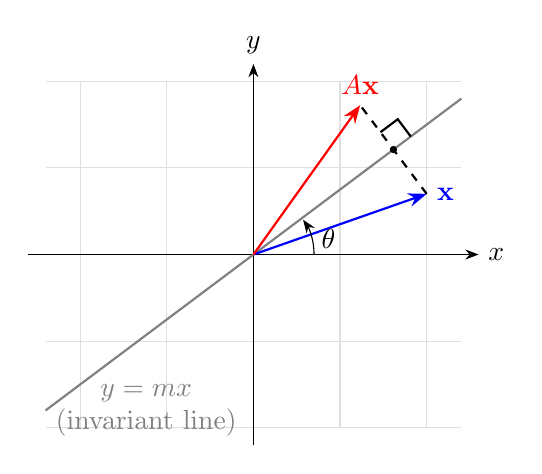
\begin{tikzpicture}[scale=2.2, >=Stealth]
	% ====== parameter ======
	\def\m{0.75} % slope of axis y=mx
	
	% ====== matrix entries for A = 1/(1+m^2)*[[1-m^2,2m],[2m,m^2-1]] ======
	\pgfmathsetmacro{\den}{1+(\m)^2}
	\pgfmathsetmacro{\a}{(1-(\m)^2)/\den}
	\pgfmathsetmacro{\b}{(2*\m)/\den}
	\pgfmathsetmacro{\c}{(2*\m)/\den}
	\pgfmathsetmacro{\d}{((\m)^2-1)/\den}
	
	% ====== choose a test vector v ======
	\pgfmathsetmacro{\vx}{1.0}
	\pgfmathsetmacro{\vy}{0.35}
	
	% ====== compute Av ======
	\pgfmathsetmacro{\wx}{\a*\vx + \b*\vy}
	\pgfmathsetmacro{\wy}{\c*\vx + \d*\vy}
	
	% ====== midpoint P = (v + Av)/2 (lies on the reflection axis) ======
	\pgfmathsetmacro{\px}{(\vx+\wx)/2}
	\pgfmathsetmacro{\py}{(\vy+\wy)/2}
	
	% ====== coordinates ======
	\coordinate (O) at (0,0);
	\coordinate (V) at (\vx,\vy);
	\coordinate (W) at (\wx,\wy);
	\coordinate (P) at (\px,\py);
	
	% ====== grid ======
	\draw[gray!25, step=0.5] (-1.2,-1.0) grid (1.2,1.0);
	
	% ====== axes ======
	\draw[->] (-1.3,0) -- (1.3,0) node[right] {$x$};
	\draw[->] (0,-1.1) -- (0,1.1) node[above] {$y$};
	
	% ====== reflection axis y=mx ======
	\draw[thick, gray]
	(-1.2,{-1.2*\m}) -- (1.2,{1.2*\m})
	node[pos=0, right, align=center] {$y=mx$\\ (invariant line)};
	
	% ====== vectors ======
	\draw[thick, blue, ->] (O) -- (V) node[pos=1, right] {$\textbf{x}$};
	\draw[thick, red,  ->] (O) -- (W) node[pos=1, above] {$A\textbf{x}$};
	
	% ====== segment from v to Av (perpendicular to axis) ======
	\draw[thick, dashed] (V) -- (W);
	
	% ===== right-angle marker at P between axis and perpendicular =====
	% axis direction u=(1,m), perpendicular direction n=(-m,1)
	\pgfmathsetmacro{\s}{0.10} % size of the marker
	
	% point along axis from P
	\coordinate (U) at ({\px+\s},{\py+\s*\m});
	% point along perpendicular from P
	\coordinate (N) at ({\px-\s*\m},{\py+\s});
	
	% build the small square: P -> U -> (U+N-P) -> N -> P
	\coordinate (C) at ({\px+\s-\s*\m},{\py+\s*\m+\s});
	\draw[thick] (U) -- (C) -- (N);
	
	\fill (P) circle (0.6pt);
	
	% ====== angle theta at origin (arc from x-axis to v) ======
%	\pgfmathsetmacro{\angv}{atan2(\vy,\vx)} % degrees
	\pgfmathsetmacro{\angv}{35} % degrees
	\pgfmathsetmacro{\r}{0.35}              % radius of the angle arc
	\draw[->] (O) ++(\r,0) arc[start angle=0, end angle=\angv, radius=\r];
	\node at ({0.55*\r*cos(\angv/2)+.25},{0.55*\r*sin(\angv/2)+.03}) {$\theta$};
	
%	% ====== matrix label ======
%	\node[align=left, anchor=west] at (0,-.5)
%	{$A=\dfrac{1}{1+m^2}\!\begin{pmatrix}
%			1-m^2 & 2m\\[2pt]
%			2m & m^2-1
%		\end{pmatrix}$};
\end{tikzpicture}
\end{document}